% Author: Calum Macewen
% Tex Author: Magdalen Berns
% Formatting: Magdalen Berns

\chapter{Fundus Photography}
\label{fundus_photography}
\lhead{\emph{Fundus Photography}}


Images of the fundus (the area encompassing the
retina, optic disc, macula, fovea and posterior pole) are a key
diagnostic tool in modern ophthalmology, allowing the practitioner
to record, revisit and compare information with ease and are used
in conjunction with the clinicians own ophthalmoscope observations.
Fundus imaging is the practice of representing the 3-D retinal
tissue layers as a 2-D image through reflecting light off of
the semi-transparent tissue layers and recording the reflected
intensities. 
There are two principal technologies used in modern ophthalmology
to obtain fundus images: the scanning \Gls{laser} ophthalmoscope
and the fundus camera. Both machines have been designed and
adapted to deal with the practical difficulties of obtaining high quality
and useful images of the retina. These two technologies deliver
diverse fields of view of the fundus and the peripheral retina, thus
providing a versatile diagnostic and prognostic tool for an ophthalmologist,
which has become necessary in the analysis and understanding of
many eye diseases.\cite{spaide2005medical}


\section{Principles of Operation}

\subsection{Fundus Camera}

The fundus camera is the original retinal imaging technology that
provided clinicians the chance to magnify the image of the retina
and record this image as a photograph via the application of indirect
ophthalmology. The modern machine comprises of an ophthalmoscopic lens,
which acts as a low power microscope, and a high performance commercially
available digital SLR camera to record the image formed through the
lens.\cite{shibata2003fundus} Fundus cameras are the standard machinery
for retinal imaging and devices are characterised by their angle of
view. The angle of view is proportional to the angular aperture and is a
measure of how much of the retina is imaged, with 30$^\circ$ considered
the normal angle of view, corresponding to around 12\% of the retina,
various angles of view are illustrated in \fref{fig:fov}.

\begin{figure}[H]
\centering
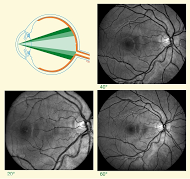
\includegraphics{figures/fieldofview}
\caption{An illustration of the standard fields of view for retinal images.\cite{saine2002ophthalmic}}
\label{fig:fov}
\end{figure}

As was mentioned in \cref{history_retinal_imaging}, the illuminating and imaging beams cannot cross paths. This is dealt with in the fundus camera by illuminating a peripheral zone of the retina with a donut of light \fref{fig:ld}. 

\begin{figure}[H]
\centering
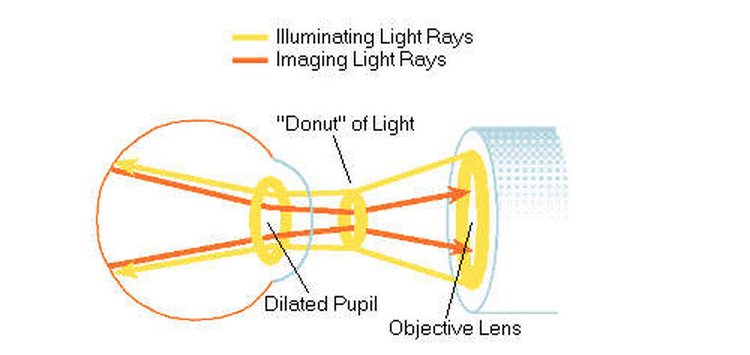
\includegraphics{figures/lightdonut}
\caption{A diagram illustrating the separation of imaging and illuminating light rays.\cite{saine2002ophthalmic}}
\label{fig:ld}
\end{figure}

This pattern is achieved by passing the illuminating rays through a series
of filters, lenses and mirrors,  which allows for imaging of the
central retinal region by way of indirect illumination. 

As discussed earlier visual impairments that necessitate correction
are commonplace. The presence of visual impairments necessitates
additional lens systems such as a dioptre compensation lens, to achieve
a focused image of the
retina. In this report we shall look specifically at the Topcon TRC-NW8F
retinal camera, shown in \fref{fig:trc}.

\begin{figure}[H]
\centering
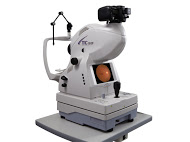
\includegraphics{figures/trc}
\caption{An image of the Topcon TRC-NW8F fundus camera.\cite{1_topconmedical.com_2015}}
\label{fig:trc}
\end{figure}


The TRC-NW8F is an efficient, highly specified multi-function fundus camera
that provides the clinician a variety of diagnostic tools, placing it at the
forefront of modern retinal imaging. By incorporating lens filters, this device
is equipped for four imaging modes (at a field of view of 45$^\circ$ with a
built-in 30$^\circ$ digital zoom feature): colour fundus, red-free, fluorescein
angiography and fundus autofluorescence, examples of each shown in \fref{fig:im}.

\begin{figure}[H]
\centering
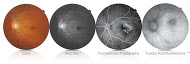
\includegraphics{figures/imagingmodes}
\caption{Comparison of the four main imaging modalities of the TRC-NW8F.\cite{1_topconmedical.com_2015}}
\label{fig:im}
\end{figure}


An important aspect of this device is the integrated auto focus, blink
detection and auto capture functionalities, making retinal imaging efficient
and easy to use. Capturing an image is a quick and comfortable process
for patients, where they simply rest their chin on the chinrest for a few
moments whilst the camera is adjusted to their eye position and focussed
on the fundus. The flash used is of low intensity to minimise patient
discomfort. The small pupil diaphragm setting on the TRC-NW8F allows
for photographs to be
taken with a pupil diameter of just 3.3mm, removing the need for mydriasis
(induced pupil dilation) in most patients. Overall this device achieves
an axial optical resolution of this device is 25$\mu m$.


\subsection{Confocal Scanning \gls{laser} Ophthalmoscope}

The \Gls{cslo} is a retinal-imaging device that utilises a \gls{laser} to illuminate a small area of the retina as
opposed to the monochromatic flash of a traditional fundus camera.
The mechanics of this instrument are shown in \fref{fig:cslo} and are as
follows: A \gls{laser} is generated and passed through a lens (L1) in order
to focus the beam on the retina. The light travels through an aperture (M1),
which separates the illuminating and reflected beams. The 2-D raster (the
scanning section) is created by firstly passing the beam through a rotating
polygon mirror (M2) (used to redirect the beam horizontally to form a line)
and then through a galvanometric mirror (M3), to form the designated 2-D
scanning area. The spherical mirror (M4) focuses the raster to a point
on the lens of the patient, which is then focused on the retina by the eye,
this then sweeps across the desired region in as little as 24 milliseconds.
The reflected light (dotted line) travelsback along a path identical to the
illuminating beam and is returned to a beam by the scanning mirrors (M2 \&
M3). The beam is split into spectral components by a beam splitter and
focused onto a photodetector by another lens (L2).\cite{webb1987confocal}

\begin{figure}[H]
\centering
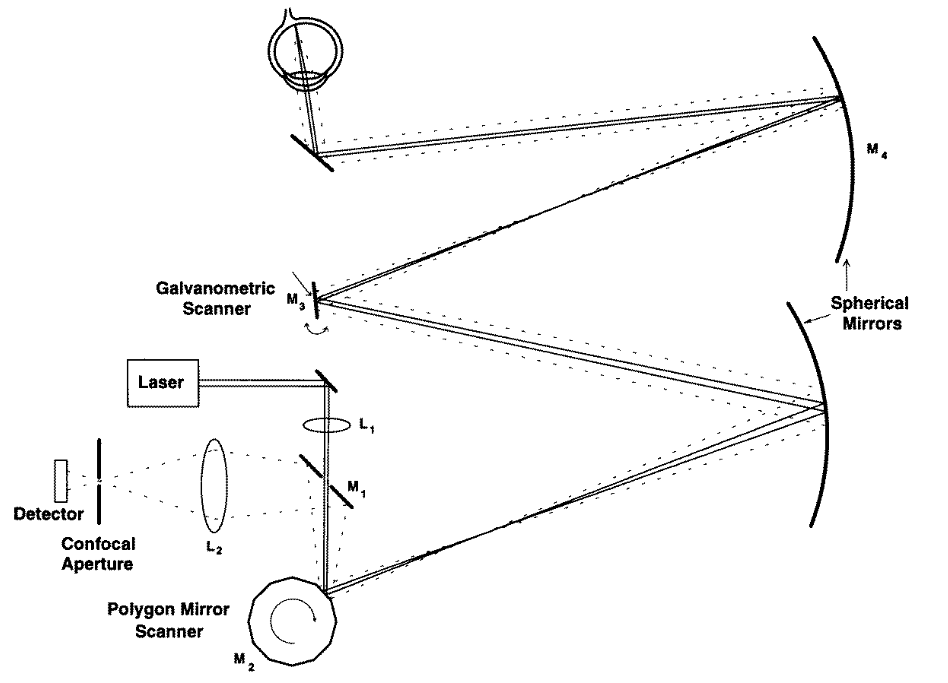
\includegraphics{figures/cslo}
\caption{Diagram showing the operating principles of a confocal \gls{laser} scanning ophthalmoscope.\cite{5_bennett_2015}}
\label{fig:cslo}
\end{figure}

Performing multiple scans and recording the signal on the photodetector
allows for the construction of a high quality image. An integral part of
this machine is the use of a confocal pinhole (small aperture) to exclude
reflected light that is not in the desired focal plane (hence this technology
is reliant on the principles of confocal microscopy). This technique (known as
optical sectioning) eliminates blurring and chromatic aberration as a specific
retinal tissue layer can be focussed on, with noise signal from other retinal
layers blocked by the aperture.\cite{sharp2004scanning} A further
ramification of confocal microscopy is the ability to create a 3-D image by
stacking many images of different focal lengths; hence an image illustrating
the structure of the optic nerve and retina can be assembled as is shown in \fref{fig:3dconfocal}.

\begin{figure}[H]
\centering
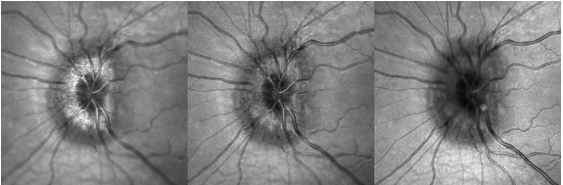
\includegraphics{figures/confocalimages}
\caption{Diagram showing how by moving the confocal plane allows for optical sectioning.\cite{sharp2004scanning}}
\label{fig:3dconfocal}
\end{figure}

As with the fundus camera \Gls{cslo}s are characterised by their field of view,
systems operate between 15$^\circ$-200$^\circ$ without requiring the use
of an invasive lens placed on the surface of the eye. Unlike the fundus
camera however the \Gls{cslo} illuminates a small circle of light with the peripheral 
donut area reflecting to form the imaging beam. A comparison between the illumination and imaging areas of a fundus camera (left image) and \Gls{cslo} (right image) are shown in  \fref{fig:illum}.

\begin{figure}[H]
\centering
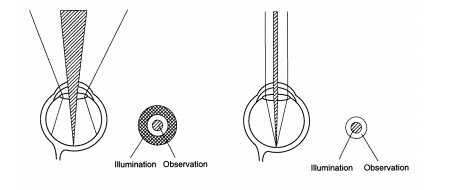
\includegraphics{figures/illumination}
\caption{An illustration of the different illumination methods used in fundus cameras (left) and \Gls{cslo} (right).\cite{5_bennett_2015}}
\label{fig:illum}
   \end{figure}

This allows for much greater light collection efficiency and permits the use
of far less intense illumination beams, hence providing a more comfortable
patient experience.\cite{5_bennett_2015} This report will focus on the Optos
California ultra-wide-field \Gls{cslo}, shown in \fref{fig:illum}.

\begin{figure}[H]
\centering
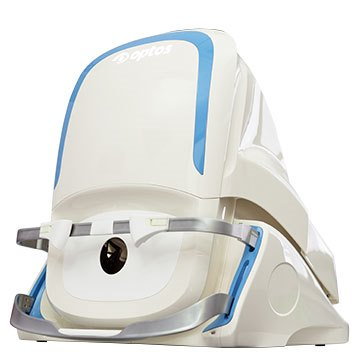
\includegraphics{figures/california}
\caption{The Optos California Ultra-Wide-Field Confocal \gls{LASER} Scanning Ophthalmoscope.\cite{1_optos.com_2015}}
\label{fig:cali}
   \end{figure}


The Optos California is a highly specified retinal-imaging device,
designed toprovide Ophthalmologists and Vitreoretinal Specialists
with a comprehensive diagnostic tool. This machine relies on the
patented Optos ultra-wide-field scanning technology, which through
the innovative use of an ellipsoidal mirror creates a virtual scanning
point inside the eye, and can generate images with a 200$^\circ$ field
of view, as shown in \fref{fig:wideview}. 

\begin{figure}[H]
\centering
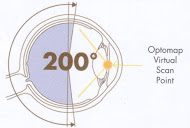
\includegraphics{figures/optoswide}
\caption{The 200$^\circ$ Optos Optomap field.\cite{1_optos.com_2015}}
\label{fig:wideview}
   \end{figure}

Through the assimilation of several \gls{laser} systems the California
has numerous imaging modalities, namely: fluorescein angiography,
fundus auto-fluorescence, ultra-wide-field colour fundus, central pole
fundus, indocyanine green angiography and red-free.\cite{7_burnett_hodd_2012} Taking images with the California is simple and quick; the patient places
their chin on the chinrest and the clinician adjusts their position with the
assistance of visual alignment software, the image is then compiled
from multiple scans and displayed on the clinicians screen in under a second. Wide-field images have an axial optical resolution of 20$\mu m$ and the
central pole fundus images have an axial optical resolution of
11$\mu m$. Images are typically obtained without the need for mydriasis
due to the optical design; hence this machine is beneficial for patients who
dilate poorly, such as diabetics. A comparison of zero dilation.\cite{11_de_brouwere_2013} images taken with a \gls{cslo} (left)
and a fundus camera (right) is shown in \fref{fig:zero}. 

\begin{figure}[H]
\centering
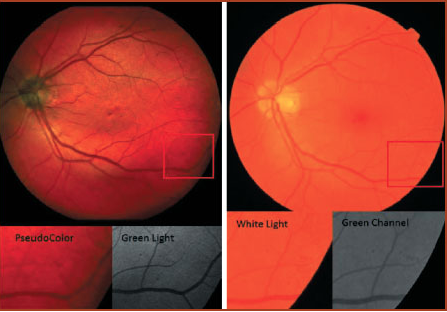
\includegraphics{figures/zerodilation}
\caption{Zero dilation images with a \gls{cslo}(left) and standard fundus camera (right).\cite{11_de_brouwere_2013}}
\label{fig:zero}
   \end{figure}


\section{Imaging Modalities and Their Diagnostic Significance}

The Optos California and Topcon TRC-NW8F are machines that house
multiple imaging modalities, with each function serving a different clinical
need. There are four main modalities: colour fundus, red-free, fluorescein angiography and fundus autofluorescence. The Optos California develops
the scope of these modalities by capturing an ultra-wide-field image;
hence this feature will be examined as a fifth modality of interest.


\subsection{Colour Fundus}

Colour fundus images focus on the retina and produce an image of the vascular
network and optic nerve head. This is the normal operating image modality for
the TRC-NW8F, where a full colour image of the retina is obtained as a result
of the white light used to illuminate the subject area, shown in \fref{fig:cf}.
The Optos California produces colour fundus images by illuminating the retina
with a green and a red \gls{laser} and combining these reflections, hence it is not
a true full spectrum colour image, as is clear from \fref{fig:cfoptos}.

\begin{figure}[H]
\centering
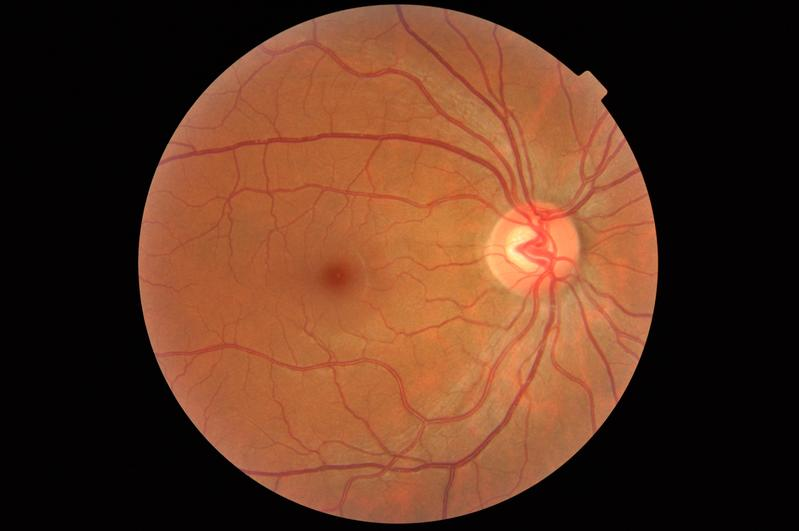
\includegraphics{figures/colourtrc}
\caption{A colour fundus image of a healthy eye, taken with the TRC-NW8F.\cite{1_topconmedical.com_2015}}
\label{fig:cf}
   \end{figure}

\begin{figure}[H]
\centering
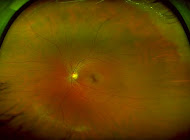
\includegraphics{figures/optoscolour}
\caption{A colour fundus image of a healthy eye, taken with the Optos California.\cite{1_optos.com_2015}}
\label{fig:cfoptos}
   \end{figure}


From a clinical perspective colour fundus imaging is the first port of call
for diagnosis of many ocular diseases, namely diabetic retinopathy, (\gls{amd}), retinal detachments and optic nerve abnormalities.\cite{3_medicine.uiowa.edu_2015} The clinician's
observations of these images direct the line of investigation, with the
majority of common ocular pathology observable in this mode. Due to
the increasing prevalence of diabetes in modern society - and thus
diabetic retinopathy - the Scottish government introduced a national diabetic screening programme to detect early signs of the disease and reduce the
likelihood of blindness and proliferation. Diabetic retinopathy is a progressive
eye disease that causes bleeding and fatty fluid leaks in the retina illustrated
in \fref{fig:dr}, which ultimately develops into \gls{dme} if
left untreated. Colour fundus images are therefore at the frontline of
diabetic retinopathy detection and are an invaluable tool in saving the vision
of many patients.

\begin{figure}[H]
\centering
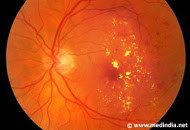
\includegraphics{figures/diabeticretinopathy}
\caption{A colour fundus image of diabetic retinopathy. The red patches indicate haemorrhages and the yellow areas show fatty fluid leakage.\cite{silva2014potential}}
\label{fig:dr}
   \end{figure}

Colour fundus images are also essential in the diagnosis of glaucoma and
papilledema, conditions that visually affect the appearance of the optic
nerve disc head.  In the case of papilledema heightened intracranial pressure
results in swelling of the optic disc, which is immediately apparent on a
fundus image, demonstrated in \fref{fig:pap}. Early diagnosis of this condition
is vital not just for preserving the vision of the patient but also in identifying
the presence of a systemic disease (papilledema is often a side effect of brain
tumours and respiratory issues). For glaucoma, colour fundus imaging is used in
the monitoring of so called \enquote{optic nerve cupping}. This is a result of increased
intraocular pressure, which causes the central section of the optic nerve (known
as the cup) to become enlarged. Ophthalmologists rely on fundus images to document the cup-to-disc ratio, which is key in assessing the efficacy of
current treatment.
\Fref{fig:cup} shows the enlargement of the cup over time.

\begin{figure}[H]
\centering
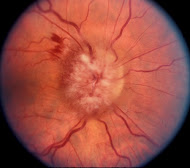
\includegraphics{figures/papilledema}
\caption{A colour fundus image of papilledema. The optic nerve head is noticeable larger and swollen.\cite{7_burnett_hodd_2012}}
\label{fig:pap}
   \end{figure}

\begin{figure}[H]
\centering
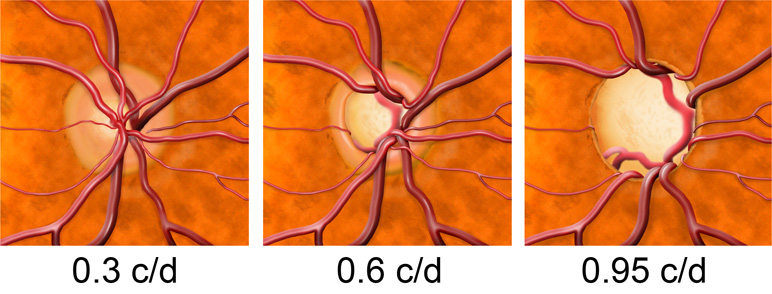
\includegraphics{figures/opticnervecupping}
\caption{An illustration of increasing cup-to-disc ratio in the optic nerve head.\cite{7_burnett_hodd_2012}}
\label{fig:cup}
   \end{figure}

	

\subsection{Red-Free}

This modality (also known as monochromatic fundus imaging) uses a monochromatic
\gls{LASER} or filtered light source to illuminate the retina. As the various retinal
tissue layers have different absorption and reflection properties one illumination
frequency can be used to highlight a specific region of interest. This technique
boosts the contrast between retinal features and provides the clinician with a
useful tool for examining individual features of the retina. Red-free specifically
relates to the use of a green filter or in the case of the Optos a green \gls{LASER},
which illuminates the retina at a wavelength of 540nm.\cite{4_bennett_2015}
A great number of visual defects and eye diseases are born from issues in
the vascular network, where clotting and lesions result in partial visual
field loss or blindness. The clinician is thus highly concerned with obtaining
images that illustrate the presence of blood in the retina, whilst minimising
noise reflections that reduce the overall image contrast. Green light is the
ideal wavelength choice for this task as it is strongly absorbed by blood,
whilst moderately reflected by the retinal pigment epithelium. This creates
high contrast images that clearly illustrate the flow of blood in the retina
as shown in \fref{fig:red} and \fref{fig:reddr}; hence this is an essential
imaging mode for practitioners, allowing simple and quick documentation of
the vascular network. Red-free is also suitable for imaging when there exists
a degree of ocular turbidity, as there is less scatter present compared with
shorter wavelengths.

\begin{figure}[H]
\centering
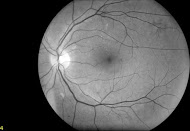
\includegraphics{figures/redfree}
\caption{A red-free image of a healthy retina.\cite{1_topconmedical.com_2015}}
\label{fig:red}
   \end{figure}

\begin{figure}[H]
\centering
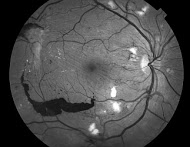
\includegraphics{figures/redfreediabetic}
\caption{A red-free image of a patient suffering from diabetic retinopathy. The large haemorrhages and fatty fluid leaks are clearly identified in this mode.\cite{1_topconmedical.com_2015}}
\label{fig:reddr}
   \end{figure}



\subsection{Fluorescein Angiography}

Fluorescein is a soluble synthetic compound used as a dye tracer in
several medical applications, principally because of its relative inertness.
As was outlined earlier, in fluorescein angiography an amount of sodium
fluorescein is injected into the patient and the resulting progression of the
dye through the vascular network is imaged or recorded over a set time
frame. The dye normally takes around 12 seconds to appear in the arteries
of the retina then after 5 seconds moves through into the capillary vessels
and veins. \Fref{fig:fluor} shows complete vascular and arterial dye diffusion.

\begin{figure}[H]
\centering
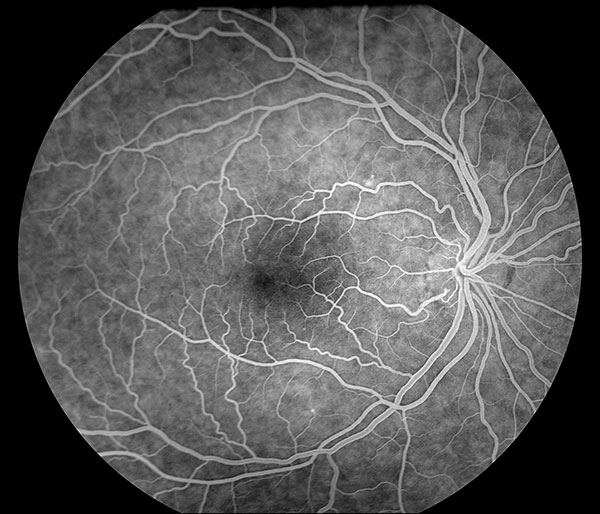
\includegraphics{figures/fluoresceinangio}
\caption{A fluorescein angiogram of a healthy eye.\cite{12_patel_2015}}
\label{fig:fluor}
   \end{figure}

Fluorescein is strongly absorbing of light with a wavelength of 494nm and
through the process of fluorescence emits light with a frequency of 520nm.
Through the use of a blue illumination light and an excitation filter high
contrast images of blood flow in the retina and choroid can be captured.
The excitation filter prevents light from being imaged with a wavelength
below 520nm thus avoids capturing any reflections from the illuminated tissue.\cite{4_bennett_2015} The clinical motivation for red-free imaging
is applicable to fluorescein angiography as they both seek to highlight the
presence of blood in the retina, with this modality capable of providing
greater detail of small capillary lesions, \fref{fig:fluordr} shows
microaneurysms symptomatic of diabetic retinopathy. Along with
illustrating vascular pathologies this modality can provide a measurement
of the patients blood flow, often used in the diagnosis of general cardiac
problems.

\begin{figure}[H]
\centering
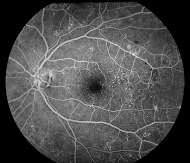
\includegraphics{figures/fadiabetic}
\caption{A fluorescein angiogram illustrating small capillary lesions in a patient suffering from diabetic retinopathy.\cite{3_medicine.uiowa.edu_2015}}
\label{fig:fluordr}
   \end{figure}

\subsection{\Gls{FAF}}

As a result of fluorescein angiography procedures ophthalmologists noticed
that areas of the fundus were fluorescent without the use of any dye tracer.
This weak autofluorescence was subsequently identified as a valuable diagnostic
criterion and plays an important role in the monitoring of disease advancement.
The method for imaging in this mode is similar to that of fluorescein angiography,
where in the case of the fundus camera an illumination beam is absorbed by
fluorescent tissue, which then emits photons of higher wavelength, allowing
for the effective filtration of insignificant reflections. \gls{cslo}s work along
the same principal but provide the additional benefit of selecting the focal
plane of interest.\cite{schmitz2008fundus} This feature is particularly relevant
for fundus autofluorescence as it removes any specious fluorescence originating
from other ocular tissue, principally the lens as it contains a small element of
fluorescent material. \cite{von1995distribution} The primary aim of this imaging
modality is to observe the accumulation of lipofuscin in the retinal pigment
epithelium, which can signal a variety of issues. Lipofuscin is fluorescent over
a broad range of wavelengths therefore the illumination beam is not as restricted
as in the case of fluorescein angiography. Recently developments have been made
with the use of near infrared illumination beams to excite melanin, providing
yet more information about the distribution of organic materials in the retina.

To understand the clinical significance of \gls{faf} imaging we must first understand
the process of lipofuscin build up.\cite{kennedy1995lipofuscin} \Gls{amd} or disease can cause photoreceptors in the retina to become
damaged and in response they will expel an outer layer of tissue, which is
subsequently absorbed by the \Gls{rpe}.\cite{spaide2003fundus}
The accretion of these molecules (or lack of) creates lipofuscin deposits
in the \Gls{rpe}, which can be used to characterise the retina either through
observing hyperfluorescence or hypofluorescence. \Fref{fig:faf} shows a
fundus autofluorescence image of a normal retina, where the natural
build up of lipofuscin in the \Gls{rpe} is clearly observed.

\begin{figure}[H]
\centering
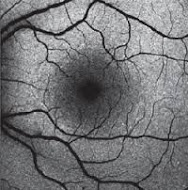
\includegraphics{figures/faf}
\caption{A confocal \gls{laser} scanning ophthalmoscope \Gls{faf} image of a normal retina. The lack of fluorescence from the macula is a result of absorbing pigmentation in this area. Retinal vessels block the reflection from the \Gls{rpe} beneath them so appear dark.\cite{1_optos.com_2015}}
\label{fig:faf}
   \end{figure}

Hyperfluorescence can be attributed to an increase in the rate
of shedding of photoreceptor outer segments or a breakdown in
the ability of the \Gls{rpe} to process these cells. Hypofluorescence
is indicative of cell death in the \Gls{rpe}, known as geographic atrophy.
\Gls{amd} results in the thinning and degradation of the \Gls{rpe} and 
so this geographic atrophy is directly observable with \gls{faf} imaging,
illustrated in \fref{fig:fafamd}.

\begin{figure}[H]
\centering
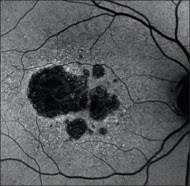
\includegraphics{figures/fafamd}
\caption{A \gls{faf} image of a patient suffering from dry \gls{amd}. \gls{amd} causes both hypo and hyperfluorescence, as a consequence of geographic atrophy and the resulting increased work of surrounding retinal tissue.\cite{2_audo_2015}}
\label{fig:fafamd}
   \end{figure}

The ability to demarcate between geographic atrophy and healthy retinal tissue makes \gls{faf} imaging a valuable prognostic tool, which is commonly used in the evaluation of treatment and the monitoring of dry \gls{amd} progression.\cite{1_murphy_2015}

\subsection{Ultra-Wide-Field Imaging}

Ultra-wide-field images greatly expand on the standard field of view and are
capable of capturing images of the peripheral retina. Until recently
non-contact imaging technology was unable to capture images with more
than a 50$^\circ$ field. \Fref{fig:uwfc} illustrates the disparity of
field of view amongst retinal imaging devices. The clinician was thus
unable to visually record any pathology directly observed in the peripheral
retina through their ophthalmoscope. Advancements in technology have opened
up this area for documentation, with peripheral retinal imaging now forming
an important part of disease detection and monitoring.\cite{8_sides_media_2015}

\begin{figure}[H]
\centering
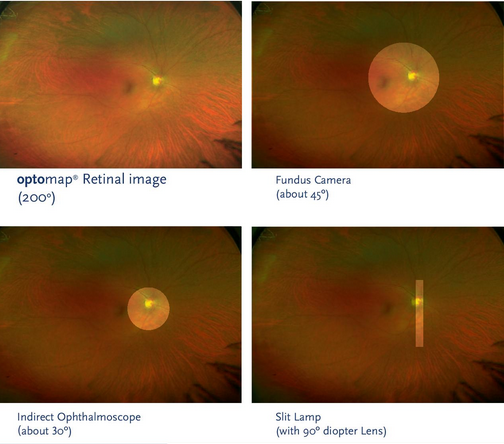
\includegraphics{figures/uwfcomparison}
\caption{A comparison of the imaging areas for various retinal imaging devices.\cite{1_optos.com_2015}}
\label{fig:uwfc}
   \end{figure}

Both the Optos California and the Topcon TRC-NW8F are capable of producing
wide-field images through differing methods. The Topcon TRC-NW8F employs
the traditional non-contact method of wide-field imaging: it sets out 9
fixation targets on the retina, takes individual photographs of each area
then pieces these photographs together using the auto-mosaic software to
give a 75$^\circ$ field. The Optos California operates in an entirely
different way, employing its patented ultra-wide-field scanning technology
to capture one complete 200$^\circ$ field. \Fref{fig:uwfvs} displays the
difference in the wide-field images these devices can capture.

\begin{figure}[H]
\centering
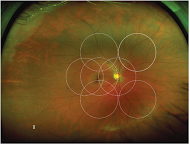
\includegraphics{figures/uwfvs}
\caption{The 200$^\circ$ Optos visual field compared with the 75$^\circ$ field of the fundus camera. Illustrative of the Optos' superiority in imaging the peripheral retina.\cite{1_optos.com_2015}}
\label{fig:uwfvs}
   \end{figure}

By combining this modality with other modalities, primarily fluorescein
angiography, the Optos presents a clear clinical advantage over other
devices. As discussed previously the progression of the dye through the
retina's circulation occurs in a short period of time; hence the piecemeal
image formation of the fundus camera is ineffectual at capturing an accurate
depiction of peripheral blood flow, as image capture is limited by the time
to move the camera. The Optos California is capable of capturing the entire
field in one image and recording a video of the dye progression through the
retina, which is of significant medical use.

From a clinical perspective the ability to capture ultra-wide-field images
is incredibly advantageous in the diagnosis of many retinal pathologies
\cite{6_witmer_kozbial_daniel_kiss_2012} and presents ophthalmologists
with a tool to detect signs that would have otherwise gone unnoticed, such
as the pathology in the far left of \fref{fig:uwfdr}.

\begin{figure}[H]
\centering
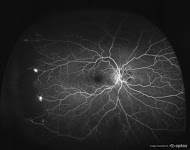
\includegraphics{figures/uwfdr}
\caption{An ultra-wide-field fluorescein angiogram of a patient suffering from diabetic retinopathy. The expanded field of view allowed for the detection of the peripheral pathology.\cite{1_optos.com_2015}}
\label{fig:uwfdr}
   \end{figure}

Recent studies have sought to evaluate the implications of ultra-wide-field
imaging for the detection and prognosis of diabetic retinopathy. One study
found that detection was increased by 17\% compared with standard fundus images,
with the classification of disease severity augmented in 9\% of cases due to the
detection of peripheral lesions. \cite{silva2014potential}


\section{Shortcomings of These Devices}


Accurate 2-D representation of the 3-D retinal tissue structure
poses a significant challenge in both devices. Images taken by the
fundus camera are centred on the posterior pole, hence they must
demonstrate to some degree the foveal depression in the centre of
the macula, along with the depth of the optic nerve head. In a standard
fundus image such as \fref{fig:standard} the dark circular area in the
centre of the image distinguishes the foveal dip, but illustrates
nothing of the actual depth of the depression. Nor does it show any
depth of the optic nerve as its reflective properties differ to that
of the surrounding retinal tissue.

\begin{figure}[H]
\centering
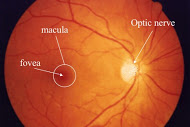
\includegraphics{figures/normalfundus}
\caption{Image showing a standard fundus image, highlighting areas of significant depth.\cite{saine2002ophthalmic}}
\label{fig:standard}
   \end{figure}

This issue resulted in the development of stereo fundoscopy, where
two similar images are taken from different positions, corresponding
to the left and right eye of the photographer, shown in \fref{fig:stereo}.
When processed these images are viewed side by side and the brain
reconstructs a 3-D image by recognising the depth differences.\cite{tyler1997stereo}
This method cannot however provide the same degree of depth perception
as in indirect ophthalmoscopy.

\begin{figure}[H]
\centering
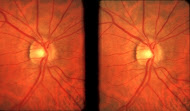
\includegraphics{figures/stereo}
\caption{Image of a stereo fundus photograph.\cite{tyler1997stereo}}
\label{fig:stereo}
   \end{figure}


In the ultra-wide-field \gls{cslo} there is the added difficulty of flattening
the curved surface without incurring a drastic reduction in proportional
accuracy, something known amongst cartographers as the \enquote{Greenland effect}.
This challenge is dealt with in the Optos California by corrective imaging
software. As the Optos California is able to perform optical sectioning it
is possible to generate a 3-D image of the retina and optic nerve by moving
the desired focal plane through the back of the eye, shown in \fref{fig:3d}.
The accuracy of these images is significantly limited by the depth resolution
of the machine, which is around 100$\mu m$, corresponding to  a large
fraction of the entire retinal thickness (300-500$\mu m$).

\begin{figure}[H]
\centering
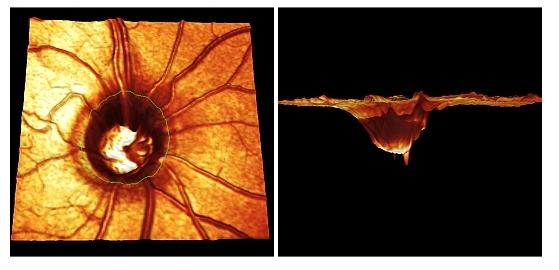
\includegraphics{figures/3dcslo}
\caption{Illustration of a 3-D image formed by confocal optical sectioning.\cite{sharp2004scanning}}
\label{fig:3d}
\end{figure}

